%pdflatex filename
\documentclass{beamer}
%\usepackage{beamerthemesplit, graphicx, colortbl}
\usepackage{graphicx, colortbl}
\usepackage{pgfpages}
\usepackage{epsfig}
\usepackage{latexsym}
\usepackage{cite}
\usepackage{amssymb}
\usepackage{xifthen}

\usetheme{Darmstadt}

\newcommand{\addressbox}{}
\newcommand{\makenote}[1]{\begin{alertblock}{}#1\end{alertblock}}
\newcommand{\makecentrednote}[1]{\begin{alertblock}{}\begin{center}#1\end{center}\end{alertblock}}
\newcommand{\titlednote}[2]{\begin{alertblock}{#1}#2\end{alertblock}}
\newcommand{\pechakucha}[2][]{%
\ifthenelse{\isempty{#1}}{\frame{\transduration{20}#2}}{\frame[#1]{\transduration{20}#2}}}

\setbeamertemplate{footline}[frame number]

\title{Testing OWL Axioms Against RDF Facts\\
A possibilistic approach}

\author{\underline{Andrea G. B. Tettamanzi}, Catherine Faron-Zucker,\\and Fabien Gandon}
\institute{Univ.\ Nice Sophia Antipolis, CNRS, INRIA, I3S, UMR 7271, France}
{
  \addressbox
}
\date{EKAW 2014, Link\"oping}
\begin{document}

%-----------

\frame{\titlepage

\includegraphics[height=.5in]{logo-unice}
\hfill

\includegraphics[height=.5in]{logo-i3s}
\hfill
\rlap{\kern.15in\raise.25in\hbox{
\includegraphics[height=.25in]{logo-cnrs}}}

\includegraphics[height=.25in]{logo-inria}
}

%\frame{\tableofcontents}

%------------------------------------------------
\section{Introduction}
\subsection[]{}

\pechakucha{
\frametitle{Introduction: Ontology Learning}
  Top-down construction of ontologies has limitations
  \begin{itemize}
    \item aprioristic and dogmatic
    \item does not scale well
    \item does not lend itself to a collaborative effort
  \end{itemize}
  Bottom-up, \emph{grass-roots} approach to ontology and KB creation
  \begin{itemize}
    \item start from RDF facts and learn OWL~2 axioms
  \end{itemize}
  Recent contributions towards OWL~2 ontology learning
  \begin{itemize}
    \item FOIL-like algorithms for learning concept definitions
    \item statistical schema induction via association rule mining
    \item light-weight schema enrichment (DL-Learner framework)
  \end{itemize}
All these methods apply and extend ILP techniques.
}

\pechakucha{
\frametitle{Introduction: Ontology validation, Axiom Scoring}
  Need for evaluating and validating ontologies
  \begin{itemize}
    \item General methodological investigations, surveys
    \item Tools like OOPS! for detecting pitfalls
    \item Integrity constraint validation
  \end{itemize}
  Ontology learning and validation rely on axiom scoring
  \begin{itemize}
    \item We tackle the problem of testing a single axiom
    \item Most popular scoring heuristics based on statistical inference
  \end{itemize}
  \begin{alertblock}{Research Questions:}
  \begin{enumerate}
    \item Can we apply a possibilistic approach to axiom testing for ontology learning?
    \item Could this be beneficial to ontology and KB validation?
  \end{enumerate}
  \end{alertblock}
}

\section{Possibilistic Axiom Scoring}

\pechakucha{
  \frametitle{Count-Based Axiom Scoring}
  Given axiom $\phi$, let us define
  \begin{description}
    \item[$u_\phi$] the support or sample size for $\phi$
    \item[$u_\phi^+$] the number of confirmations of $\phi$
    \item[$u_\phi^-$] the number of counterexamples (falsifiers) of $\phi$
  \end{description}
  Score from statistical inference: $\Pr(\mbox{$\phi$ is true}\mid\mbox{evidence})$
  \begin{itemize}
    \item Simple statistics: $\hat{p}_\phi = u_\phi^+/u_\phi$
    \item Refinements are possible, e.g., confidence intervals
  \end{itemize}

  \makenote{Implicit assumption that we know how to estimate $\Pr(e \mid \phi)$ in
  \[
    \Pr(\phi \mid e) =
      \frac{\Pr(e \mid \phi)\Pr(\phi)}{\Pr(e \mid \phi)\Pr(\phi) + \Pr(e \mid \neg\phi)\Pr(\neg\phi)}
  \]}
  $\Rightarrow$ Alternative scoring heuristics based on possibility theory,
  weaker than probability theory
}

\subsection{Possibility Theory}

\pechakucha{\frametitle{Possibility Theory}
  \begin{definition}[Possibility Distribution]
    \[
      \pi: \Omega \to [0, 1]
    \]
  \end{definition}
  \begin{definition}[Possibility and Necessity Measures]
    \vspace{-1em}
    \begin{eqnarray*}
      \Pi(A) &=& \max_{\omega\in A} \pi(\omega); \\
      N(A)   &=& 1 - \Pi(\bar{A}) = \min_{\omega\in \bar{A}} \{1 - \pi(\omega)\}.
    \end{eqnarray*}
  \end{definition}

For all subsets $A\subseteq \Omega$,
\begin{enumerate}
%  \item $\Pi(A \cup B) = \max\{\Pi(A), \Pi(B)\}$;
%  \item $\Pi(A \cup \bar A) = \max\{\Pi(A), \Pi(\bar A)\}=1$;
  \item $\Pi(\emptyset) = N(\emptyset) = 0$,\quad $\Pi(\Omega) = N(\Omega) = 1$;
%  \item $N(A \cap B) = \min\{N(A), N(B)\}$;
  \item $\Pi(A) = 1 - N(\bar{A})$ (duality);
%  \item $N(A) \leq \Pi(A)$;
  \item $N(A) > 0$ implies $\Pi(A) = 1$,\quad $\Pi(A) < 1$ implies $N(A) = 0$.
\end{enumerate}
In case of complete ignorance on $A$, $\Pi(A) = \Pi(\bar{A}) = 1$.
}

\subsection{Support of an Axiom}

\pechakucha{\frametitle{Support of an Axiom}
  $\mathrm{BS}$: finite set of \emph{basic statements}, i.e.,\\
  assertions that may be tested by a SPARQL \texttt{ASK} query.

  \begin{definition}[Content of Axiom $\phi$]
    \[
      \mathrm{content}(\phi) = \{\psi : \phi \models \psi\} \cap \mathrm{BS}.
    \]
  \end{definition}
  \begin{itemize}
  \item $\mathrm{content}(\phi)$ is finite \quad $\Leftarrow$ \quad $\mathrm{BS}$ is finite
  \item every $\psi \in \mathrm{content}(\phi)$ may be tested by a SPARQL \texttt{ASK} query
  \end{itemize}

  \vfill
  \begin{definition}[Support of Axiom $\phi$]
    \[
      u_\phi = |\mathrm{content}(\phi)|.
    \]
  \end{definition}
}

\subsection{Possibility and Necessity of an Axiom}

\pechakucha{\frametitle{Possibility and Necessity of an Axiom}
\begin{eqnarray*}
  \Pi(\phi) &=& 1 - \sqrt{1 - \left(\frac{u_\phi - u_\phi^-}{u_\phi}\right)^2} \\
  N(\phi) &=& \sqrt{1 - \left(\frac{u_\phi - u_\phi^+}{u_\phi}\right)^2}\quad
    \mbox{if $\Pi(\phi) = 1$, 0 otherwise.}
\end{eqnarray*}
%
  \begin{center}
    \begin{tabular}{cc}
      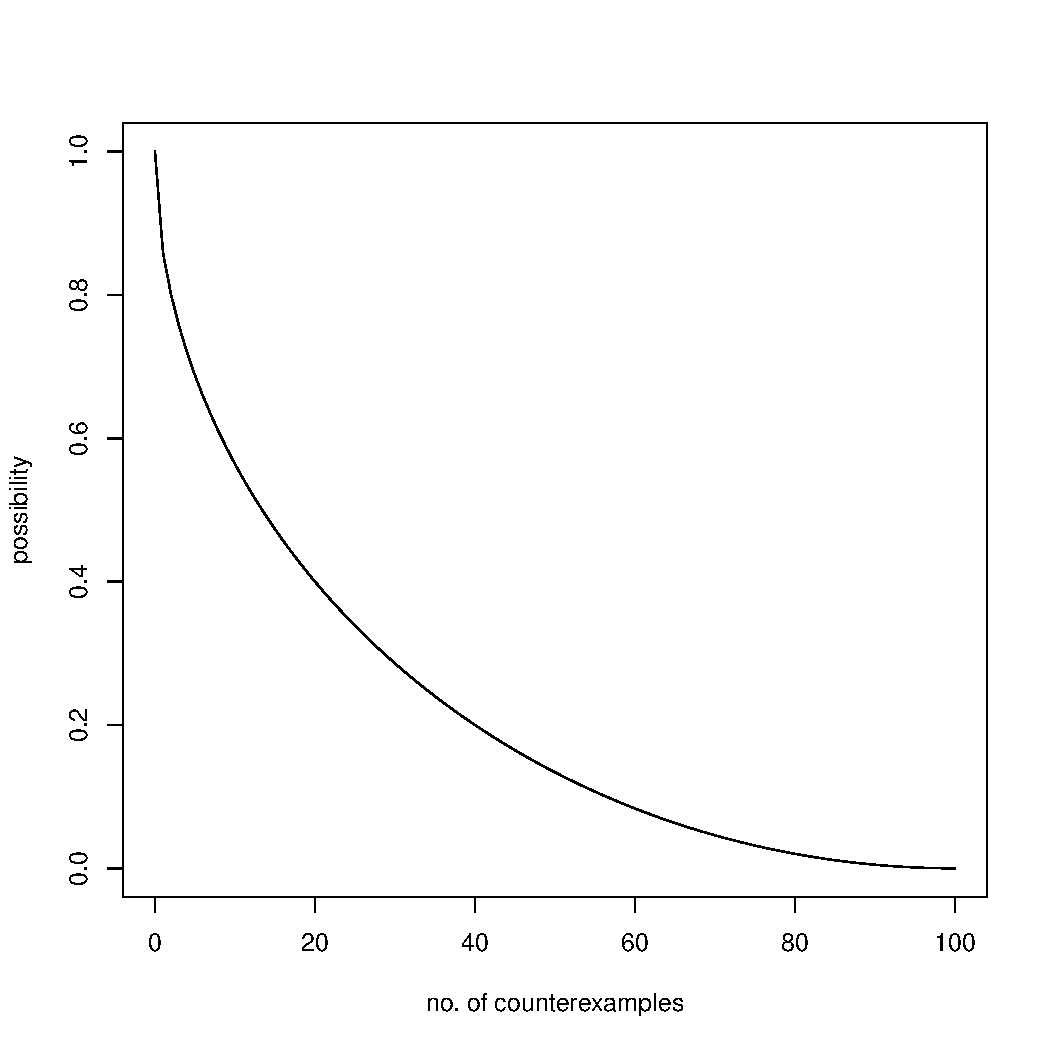
\includegraphics[width=1.4in]{../possibility} &
      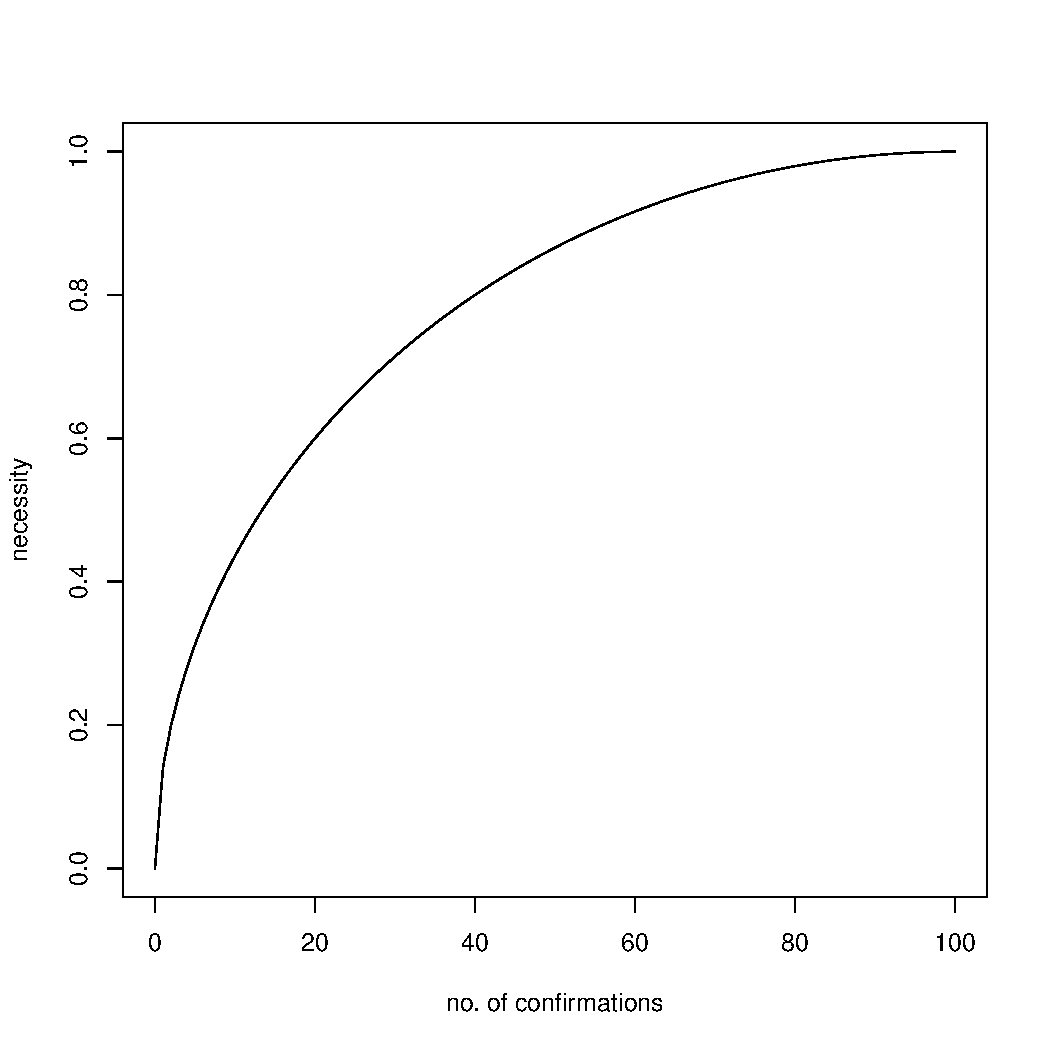
\includegraphics[width=1.4in]{../necessity}
    \end{tabular}
  \end{center}
}

\pechakucha{\frametitle{Acceptance/Rejection Index}
  Combination of possibility and necessity of an axiom:
  \begin{definition}
    \[
      \mathrm{ARI}(\phi) = N(\phi) - N(\neg\phi) = N(\phi) + \Pi(\phi) - 1
    \]
  \end{definition}
  \begin{itemize}
  \item $-1 \leq \mathrm{ARI}(\phi) \leq 1$ for all axiom $\phi$
  \item $\mathrm{ARI}(\phi)<0$ suggests rejection of $\phi$ ($\Pi(\phi)<1$)
  \item $\mathrm{ARI}(\phi)>0$ suggests acceptance of $\phi$ ($N(\phi)>0$)
  \item $\mathrm{ARI}(\phi)\approx0$ reflects ignorance about the status of $\phi$
  \end{itemize}
}

\section{Candidate Axiom Testing}
\subsection[]{}

\pechakucha{\frametitle{OWL~2 $\to$ SPARQL}
To test axioms, we define a mapping $Q(E, x)$ from OWL~2 expressions to SPARQL graph patterns
such that
\begin{center}
\texttt{SELECT DISTINCT ?x WHERE \{} $Q(E, \mbox{\tt ?x})$ \texttt{\}}
\end{center}
returns $[Q(E, x)]$, all known instances of class expression $E$
and
\[
  \mbox{\tt ASK \{ } Q(E, a) \mbox{\tt\ \}}
\]
checks whether $E(a)$ is in the RDF base.

\vfill
  \begin{exampleblock}{For an atomic concept $A$ (a valid IRI),}
    \[
      Q(A, \mbox{\tt ?x}) = \mbox{\tt ?x a }A\mbox{\tt~.}
    \]
  \end{exampleblock}
}

\subsection[]{Concept Negation}

\pechakucha{\frametitle{Concept Negation: $Q(\neg C, \mbox{\tt ?x})$}
  \begin{exampleblock}{}\vspace{-0.5em}
    \begin{equation}\label{eq:neg-as-failure}
      Q(\neg C, \mbox{\tt ?x}) =
      \begin{minipage}[t]{5in}
        \begin{tabbing}
          \quad\=\quad\=\quad\=\kill
          \{\>\texttt{?x ?p ?o .}\\
            \>\texttt{FILTER NOT EXISTS} Q(C, \mbox{\tt ?x}) \mbox{\tt\ \}}
        \end{tabbing}
      \end{minipage}
    \end{equation}
  \end{exampleblock}
  has the problem of treating negation as failure.

  \begin{exampleblock}{}\vspace{-0.5em}
    \begin{equation}\label{eq:approx-open-world-negation}
      Q(\neg C, \mbox{\tt ?x}) =
      \begin{minipage}[t]{5in}
        \begin{tabbing}
          \quad\=\quad\=\quad\=\kill
          \{\>\texttt{?x a ?dc .}\\
            \>\texttt{FILTER NOT EXISTS} \{\\
            \>\>\texttt{?z a ?dc . } $Q(C, \mbox{\tt ?z})$\ \}\\
          \}
        \end{tabbing}
      \end{minipage}
    \end{equation}
  \end{exampleblock}
  Better than (\ref{eq:neg-as-failure}), but just pushes the problem one step further

  \begin{exampleblock}{}\vspace{-1.5em}
    \begin{equation}\label{eq:negation-with-disjointWith}
      Q(\neg C, \mbox{\tt ?x}) =
        \mbox{\tt \{ ?x a ?dc .\ ?dc owl:disjointWith }
        C \mbox{\tt\ \}}
    \end{equation}
  \end{exampleblock}
  OK, but very few \textsf{DisjointClasses} axioms currently found in ontologies!
}

\pechakucha{\frametitle{Concept Negation: Discussion}
  \begin{center}
    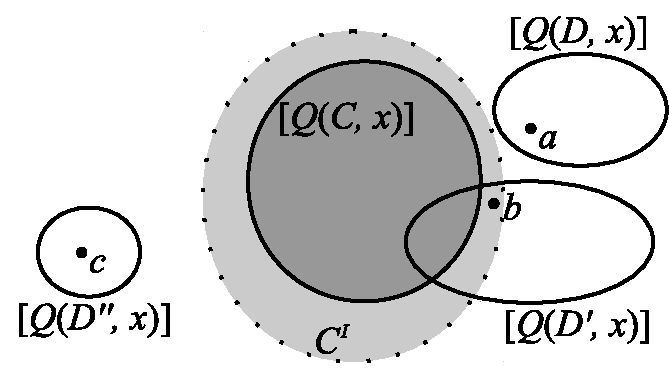
\includegraphics[height=2in]{../negation}
  \end{center}
}

\section{Subsumption Axiom Testing}
\subsection[]{}

\pechakucha{\frametitle{$\mathsf{SubClassOf}(C\ D)$ Axioms}
  To test \textsf{SubClassOf} axioms, we must define their logical content
  based on their OWL~2 semantics:
\begin{eqnarray*}
  (C \sqsubseteq D)^\mathcal{I} &=& C^\mathcal{I} \subseteq D^\mathcal{I} \\
  &\equiv& \forall x\quad x \in C^\mathcal{I} \Rightarrow x \in D^\mathcal{I}
\end{eqnarray*}

Therefore,
\begin{block}{}
\[
  \mathrm{content}(C \sqsubseteq D) = \{D(a) : \mbox{$C(a)$ is in the RDF store} \}
\]
\end{block}
because, if $C(a)$ holds,
\[
  C(a) \Rightarrow D(a) \equiv \neg C(a) \lor D(a) \equiv \top \lor D(a) \equiv D(a)
\]
}

\pechakucha{\frametitle{Support, Confirmations and Counterexamples of $C \sqsubseteq D$}
$u_{C \sqsubseteq D}$ can be computed by
\[
  \begin{minipage}[c]{5in}
    \begin{tabbing}
      \quad\=\quad\=\quad\=\kill
      \texttt{SELECT (count(DISTINCT ?x) AS ?u)}
      \texttt{WHERE} \{$Q(C, \mbox{\tt ?x})$\}.
    \end{tabbing}
  \end{minipage}
\]
As for the computational definition of $u^+_{C \sqsubseteq D}$ and $u^-_{C \sqsubseteq D}$:
\begin{itemize}
\item confirmations: $a$ s.t.\ $a \in [Q(C, x)]$ and $a \in [Q(D, x)]$;
\item counterexamples: $a$ s.t.\ $a \in [Q(C, x)]$ and $a \in [Q(\neg D, x)]$.
\end{itemize}
Therefore,
\begin{itemize}
\item $u^+_{C \sqsubseteq D}$ can be computed by
\[
  \begin{minipage}[c]{5in}
    \begin{tabbing}
      \quad\=\quad\=\quad\=\kill
      \texttt{SELECT (count(DISTINCT ?x) AS ?numConfirmations)}\\
      \texttt{WHERE} \{ $Q(C, \mbox{\tt ?x})$ $Q(D, \mbox{\tt ?x})$ \}
    \end{tabbing}
  \end{minipage}
\]
\item $u^-_{C \sqsubseteq D}$ can be computed by
\[
  \begin{minipage}[c]{5in}
    \begin{tabbing}
      \quad\=\quad\=\quad\=\kill
      \texttt{SELECT (count(DISTINCT ?x) AS ?numCounterexamples)}\\
      \texttt{WHERE} \{ $Q(C, \mbox{\tt ?x})$ $Q(\neg D, \mbox{\tt ?x})$ \}
    \end{tabbing}
  \end{minipage}
\]
\end{itemize}
}

\subsection{Experiments \& Results}

\pechakucha{\frametitle{Experiments}
Experimental Setup:
\begin{itemize}
\item DBpedia 3.9 in English as RDF fact repository
\item Local dump (812,546,748 RDF triples) loaded into Jena TDB
\item Method coded in Java, using Jena ARQ and TDB
\item 12 6-core Intel Xeon CPUs @2.60GHz (15,360 KB cache),
128 GB RAM, 4 TB HD (128 GB SSD cache),
Ubuntu 64-bit OS.
\end{itemize}

Two experiments:
\begin{enumerate}
\item Explorative test of systematically generated subsumption axioms
\item Exhaustive test of all subsumption axioms in the DBpedia ontology.
\end{enumerate}
Results at \url{http://www.i3s.unice.fr/~tettaman/RDFMining/}.
}

\pechakucha{\frametitle{Explorative Experiment}
Systematically generate and test SubClassOf axioms involving atomic classes only
\begin{itemize}
\item For each of the 442 classes $C$ referred to in the RDF store
\item Construct all $C \sqsubseteq D$ : $C$ and $D$ share at least one instance
\item Classes $D$ are obtained with query
\begin{center}
  \texttt{SELECT DISTINCT ?D WHERE \{}$Q(C, \mbox{\tt ?x})$. \texttt{?x a ?D\}}
\end{center}
\end{itemize}
Due to the sheer number of axioms thus generated and to the long time
it takes to test them, this experiment is still underway
}

\pechakucha{\frametitle{Explorative Experiment: Test Time}
\begin{center}
  \begin{tabular}{cc}
    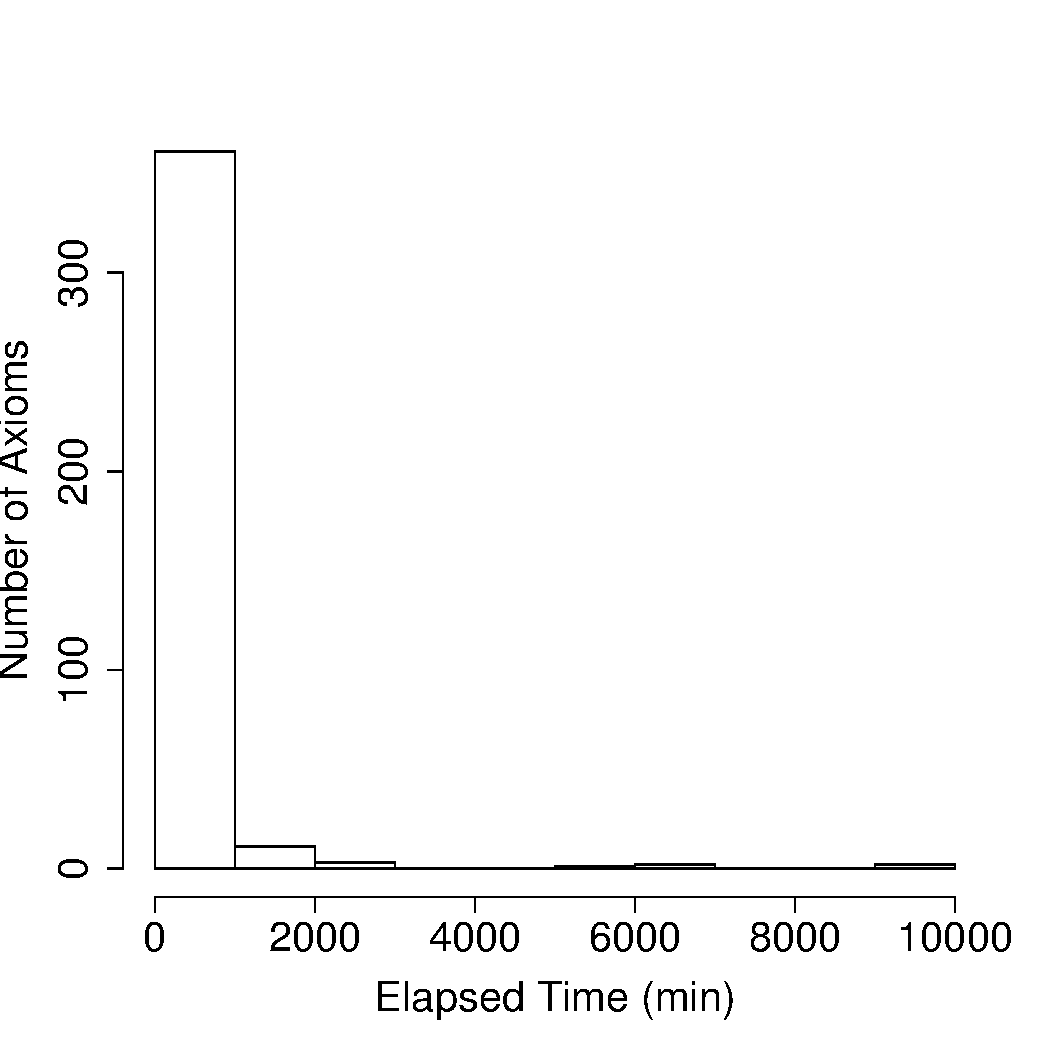
\includegraphics[height=2in]{systematic-time-hist} &
    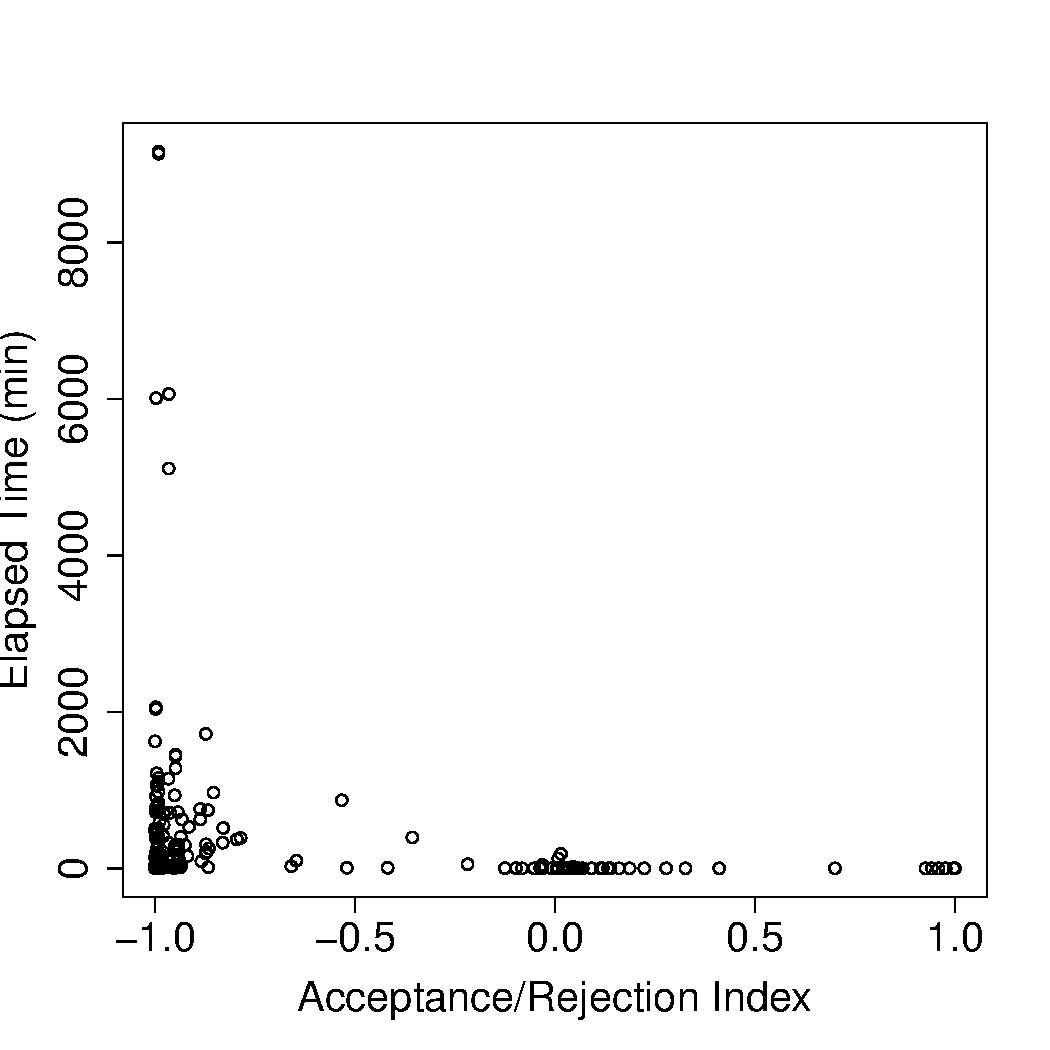
\includegraphics[height=2in]{time-ARI}
  \end{tabular}
\end{center}
Time to test an axiom inversely proportional to its $\mathrm{ARI}$

Good news: time-out on test $\Rightarrow$ $\mathrm{ARI}(\phi) < 0$ likely!
}

\pechakucha{\frametitle{Explorative Experiment: Results}
Assessment:
\begin{enumerate}
\item sort the 380 tested axioms by their ARI
\item manually tag each of them as either \emph{true} or \emph{false}
\end{enumerate}

Findings:
\begin{itemize}
\item $\mathrm{ARI}(\phi)>1/3$ as the optimal acceptance criterion for $\phi$
\item This would yield 4 FP and 6 FN (97.37\% accuracy)
\item Misclassifications to blame on mistakes in DBpedia
\item Pr score w/ 0.7 threshold yields 13 FN (+7) and 4 FP (=)
\end{itemize}
}

\pechakucha{\frametitle{Explorative Experiment: Comparison w/ Probabilistic Score}
\begin{center}
  \begin{tabular}{cc}
    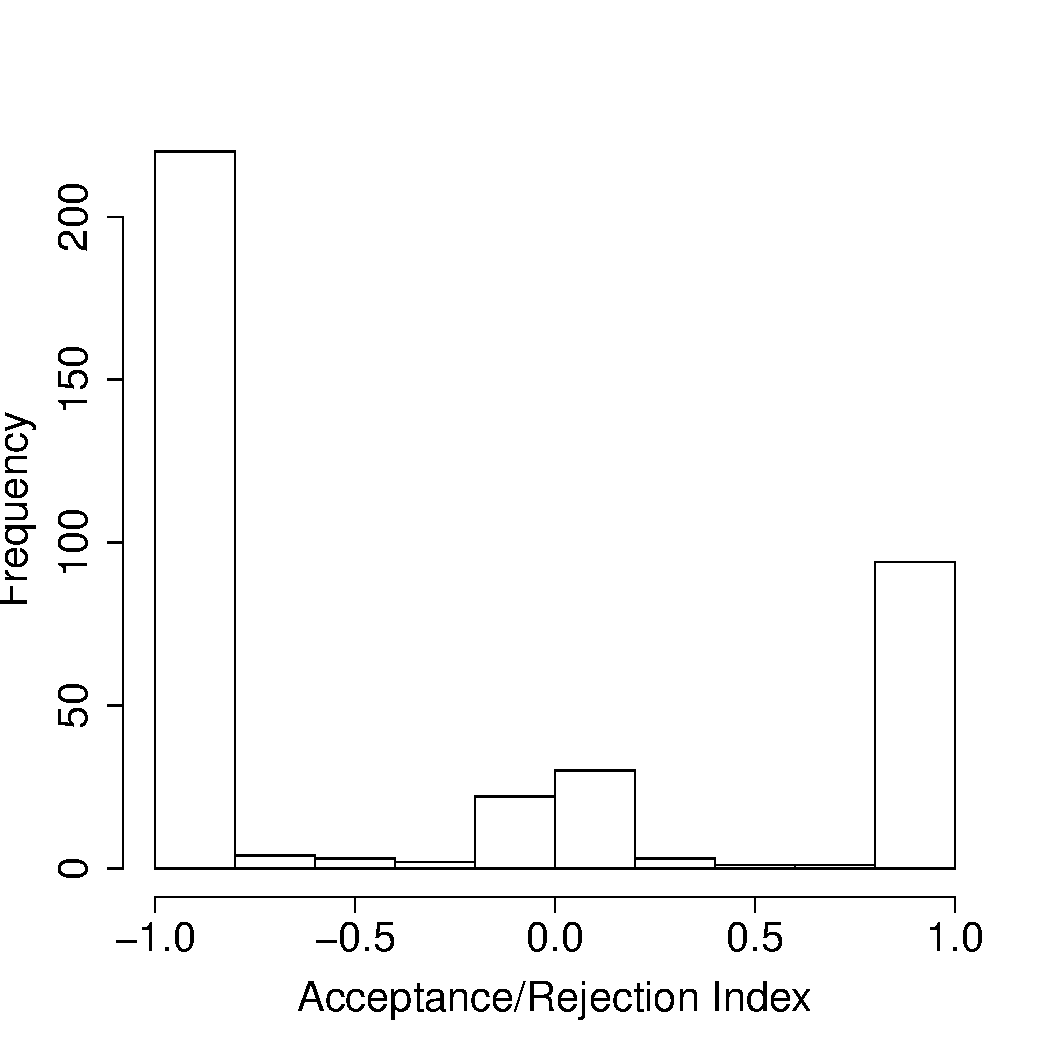
\includegraphics[height=2in]{ARI-hist} &
    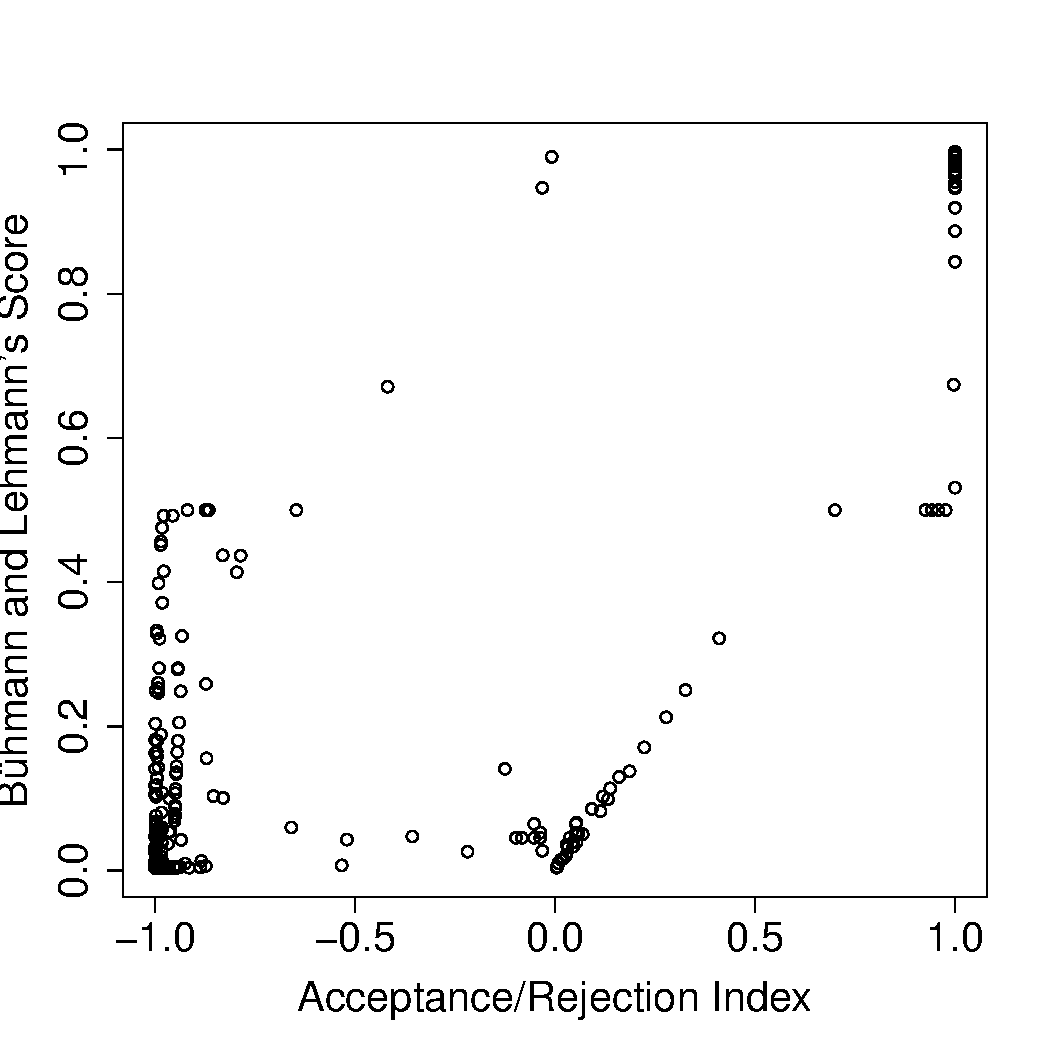
\includegraphics[height=2in]{ARI-BLS}
  \end{tabular}
\end{center}
}

\pechakucha{\frametitle{Exhaustive Experiment}
Test all \textsf{SubClassOf} axioms in DBpedia ontology
\begin{itemize}
\item Functional syntax, with query
\begin{tabbing}
\texttt{SELECT DISTINCT}\\
\quad\texttt{concat(}\=\texttt{"SubClassOf(<", str(?x),}\\
\>\texttt{"> <",str(?y),">)")}\\
\texttt{WHERE \{ ?x a owl:Class . ?x rdfs:subClassOf ?y \}}
\end{tabbing}
\item 541 axioms
\item Testing ``only'' took 1 h 23 min 31 s
\end{itemize}
}

\pechakucha{\frametitle{Exhaustive Experiment: Results}
\begin{itemize}
  \item For 143 axioms, $u_\phi = 0$ (empty content!): $\mathrm{ARI}(\phi)=0$
  \item For 28 axioms, $\mathrm{ARI}(\phi)<0$ $\Rightarrow$ $\exists$ erroneous facts
\end{itemize}
Examples of axioms $C \sqsubseteq D$ with their conterexamples:
\begin{center}\scriptsize
  \begin{tabular}{|l|l|} \hline
  \textbf{Axiom} & \textbf{Counterexamples} \\ \hline
$\mbox{\textsf{dbo:LaunchPad}} \sqsubseteq \mbox{\textsf{dbo:Infrastructure}}$ & \textsf{:USA} \\ \hline
$\mbox{\textsf{dbo:Brain}} \sqsubseteq \mbox{\textsf{dbo:AnatomicalStructure}}$ & \textsf{:Brain} [\emph{sic}] \\ \hline
$\mbox{\textsf{dbo:Train}} \sqsubseteq \mbox{\textsf{dbo:MeanOfTransportation}}$ &
  \textsf{:New\_Jersey\_Transit\_rail\_op\-er\-ations}, \\
& \textsf{:ALWEG} \\ \hline
$\mbox{\textsf{dbo:ProgrammingLanguage}} \sqsubseteq \mbox{\textsf{dbo:Software}}$ & \textsf{:Ajax} \\ \hline
$\mbox{\textsf{dbo:PoliticalParty}} \sqsubseteq \mbox{\textsf{dbo:Organisation}}$ &
  \textsf{:Guelphs\_and\_Ghibellines}, \textsf{:-}, \\
& \textsf{:New\_People's\_Army}, \textsf{:Syrian}\\
\hline
  \end{tabular}
\end{center}

N.B.: counterexamples are instances $a$ such that $C(a)$ and
$E(a)$ with $E^\mathcal{I} \cap D^\mathcal{I} = \emptyset$:
in this case, either $C(a)$ is wrong or $E(a)$ is.
}

\section{Conclusion}
\subsection[]{}

\pechakucha{\frametitle{Conclusions \& Future Work}

Contributions
\begin{itemize}
\item Axiom scoring heuristics based on possibility theory
\item Solid basis for axiom induction, ontology learning
\item A framework based on the proposed heuristics
\end{itemize}

The proposed heuristics
\begin{itemize}
\item is suitable for axiom induction
\item may be useful for ontology and KB validation
\item no less rigorous or objective than probability-based scoring
\end{itemize}

Future work
\begin{itemize}
\item extend experimental evaluation to more general axioms
\item enlarge test base w/ additional RDF datasets from the LOD
\item improve framework by setting a time-out on query evaluation
\end{itemize}
}

\frame{\frametitle{The End}
  \makenote{\huge Thank you for your attention!}
}

\end{document}
